\noindent
\begin{minipage}[t]{0.48\columnwidth}
\captionof{listing}{Comprehension example}
\label{code:comprehension-example}
\begin{minted}[
  fontsize=\scriptsize,
  baselinestretch=0.95,
  breaklines,
  breakanywhere
]{json}
{
  "book": "1984",
  "query": "What are the three slogans of the Party?",
  "ground_truth": "WAR IS PEACE, FREEDOM IS SLAVERY, IGNORANCE IS STRENGTH"
}
\end{minted}
\end{minipage}\hfill
\begin{minipage}[t]{0.48\columnwidth}
\captionof{listing}{Spoiler-prevention example}
\label{code:spoiler-example}
\begin{minted}[
  fontsize=\scriptsize,
  baselinestretch=0.95,
  breaklines,
  breakanywhere
]{json}
{
  "book": "1984",
  "query": "What happens to the glass paperweight Winston bought?",
  "percentage_of_book_read": 55,
  "evaluation_rules": {
    "forbidden_keywords": ["smashed","pieces","hearth-stone","fragment of coral"]
  }
}
\end{minted}
\end{minipage}


We evaluated a total of $600$ queries across three literary novels, (i) 1984 (George Orwell)~\cite{b31}, (ii) Of Mice and Men (John Steinbeck)~\cite{b32}, and (iii) The Death of Ivan Ilych (Leo Tolstoy)~\cite{b33}, using both technical and LLM-judged metrics.
The benchmark included 300 comprehension queries (30 queries per model across 10 models) in the format as shown in Code~\ref{code:comprehension-example}, and 300 spoiler prevention scenarios (30 queries per model across 10 models), in the format shown in  Code~\ref{code:spoiler-example}.
Each comprehension item paired a short reference answer generated with \texttt{Gemini 2.5 Pro}, while spoiler tasks defined “forbidden facts” with progress-based thresholds.
For every item, passages were retrieved through hybrid lexical–semantic search, deduplicated, and limited to six excerpts.
The models were instructed to answer only from the excerpts and to respond “Info not available in text so far” when necessary.
Responses were generated with temperature $0.3$.

\begin{figure}[!t]
  \centering
  \begin{minipage}[t]{0.48\columnwidth}
    \centering
    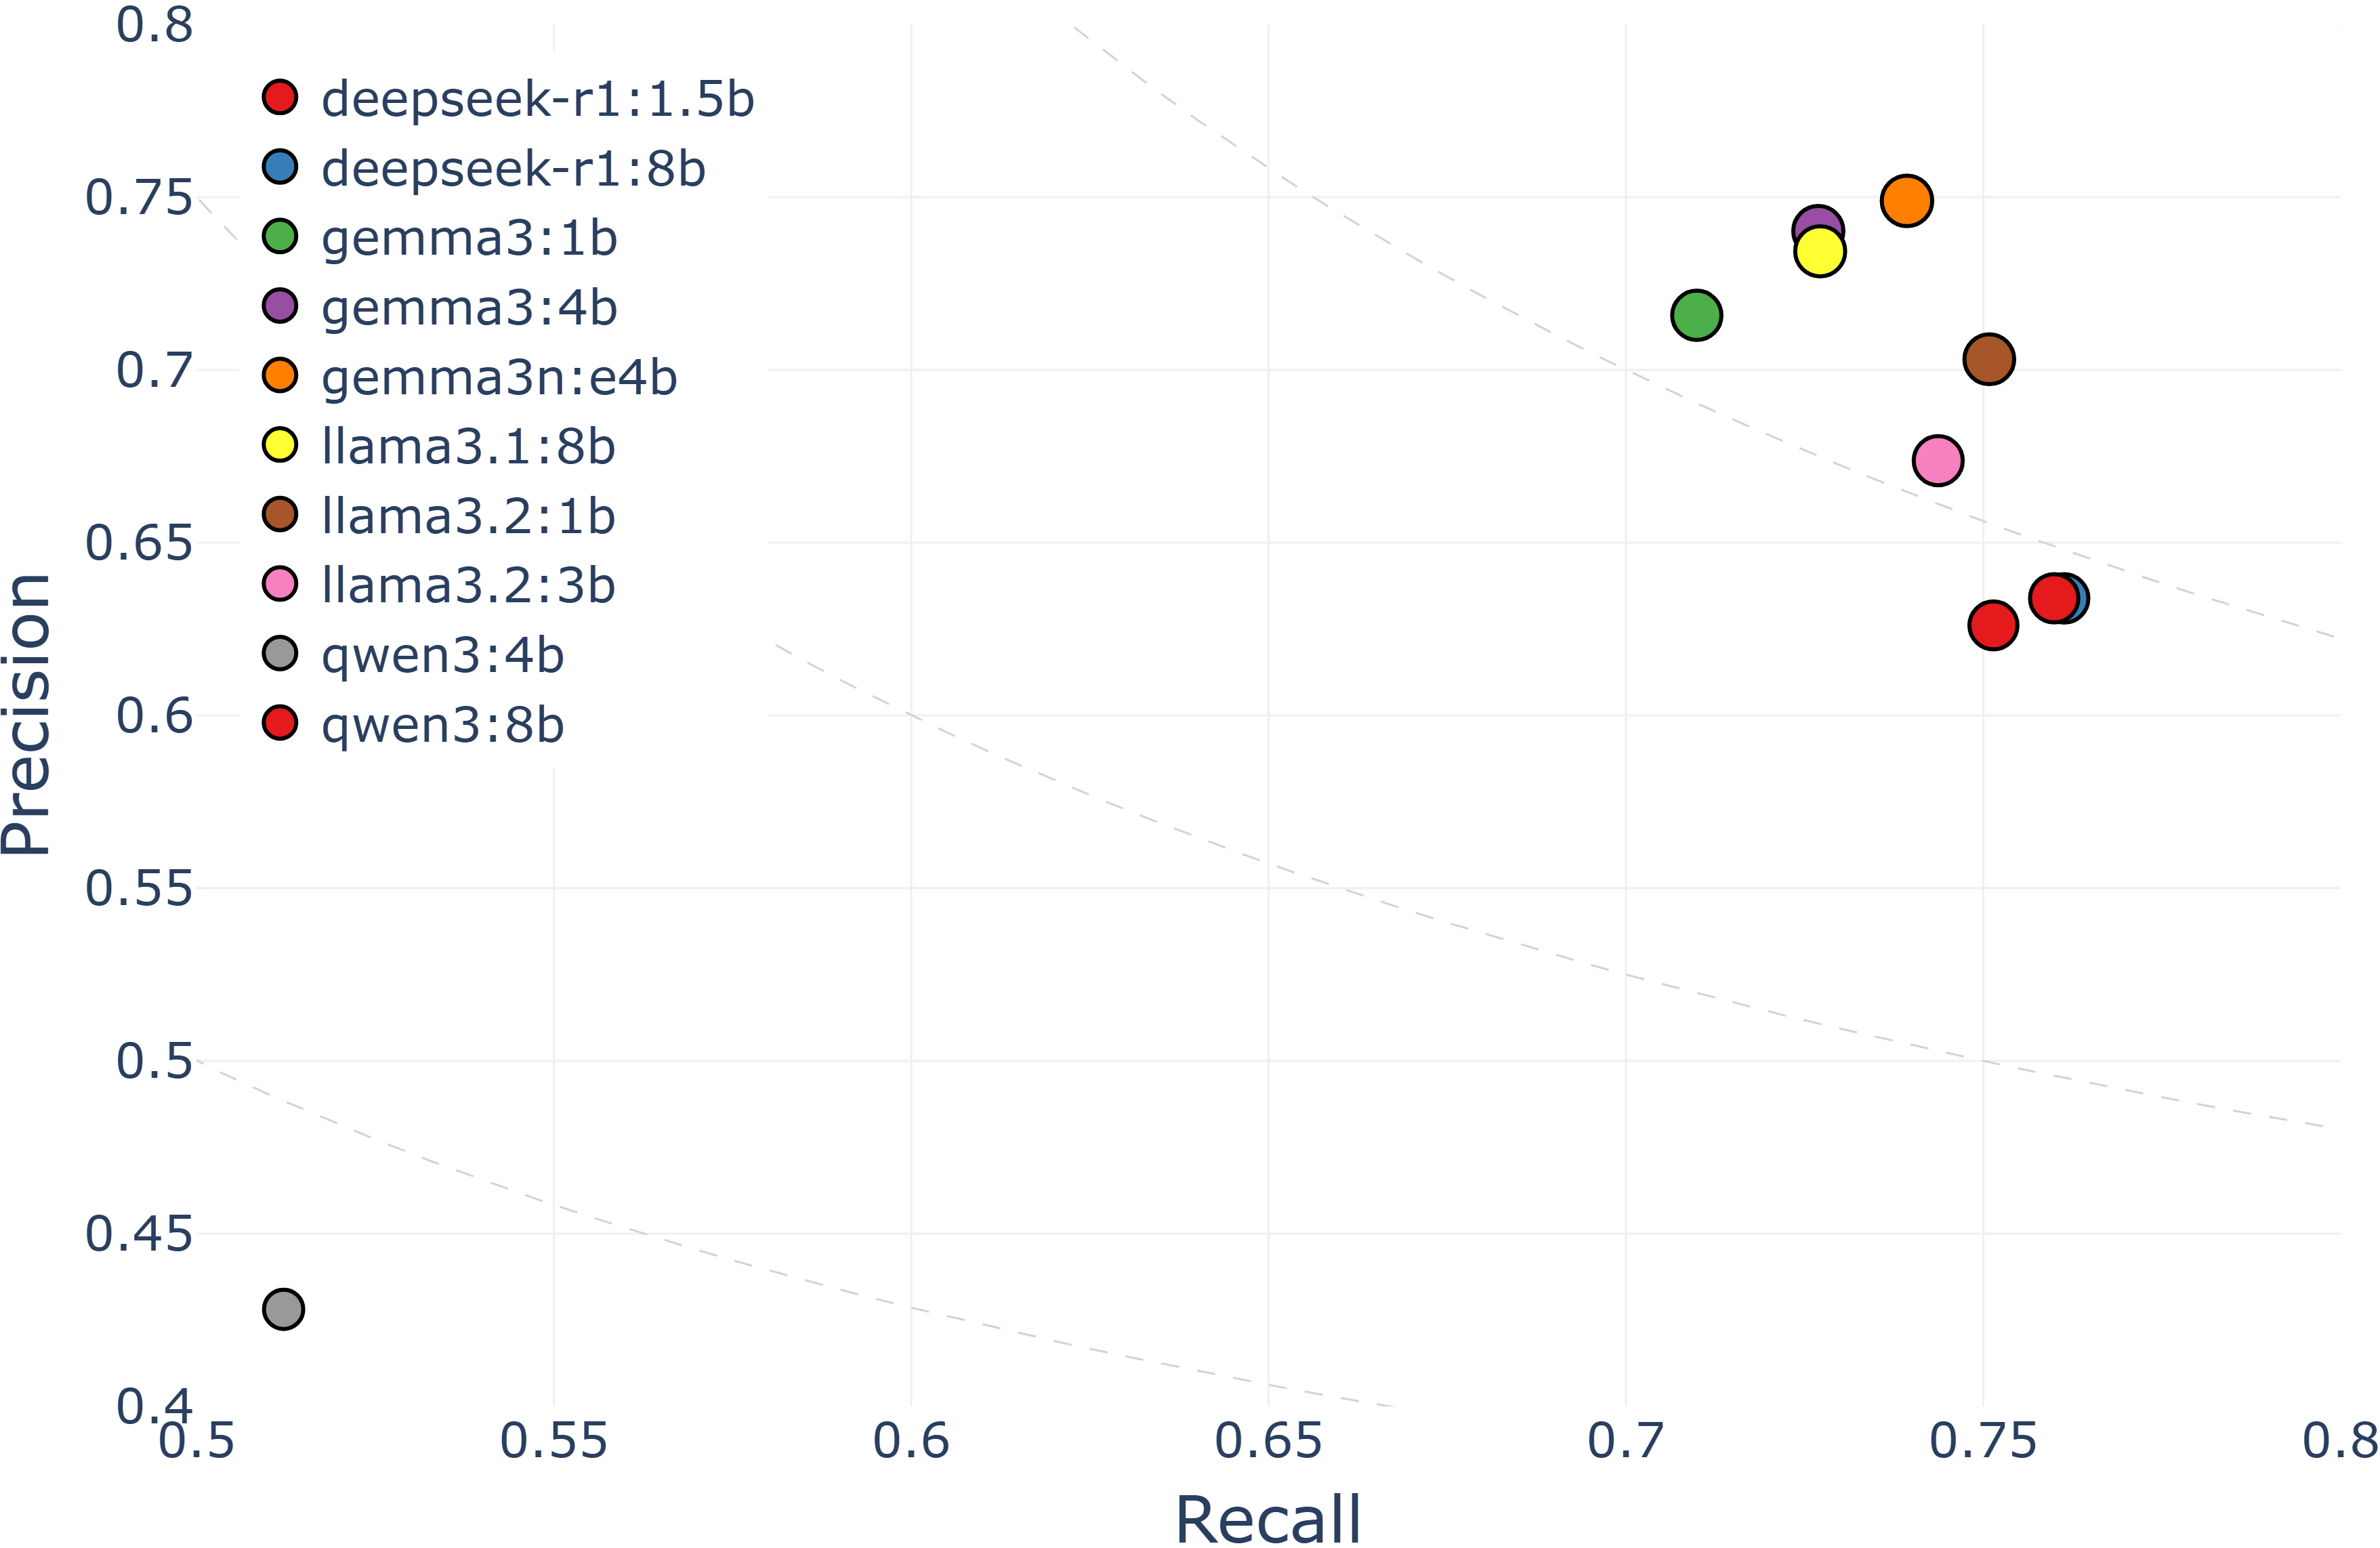
\includegraphics[width=\linewidth]{images/01_precision_recall_plane.png}
    \caption{Precision Recall Plane}
    \label{fig:eval_precision_recall}
  \end{minipage}\hfill
  \begin{minipage}[t]{0.48\columnwidth}
    \centering
    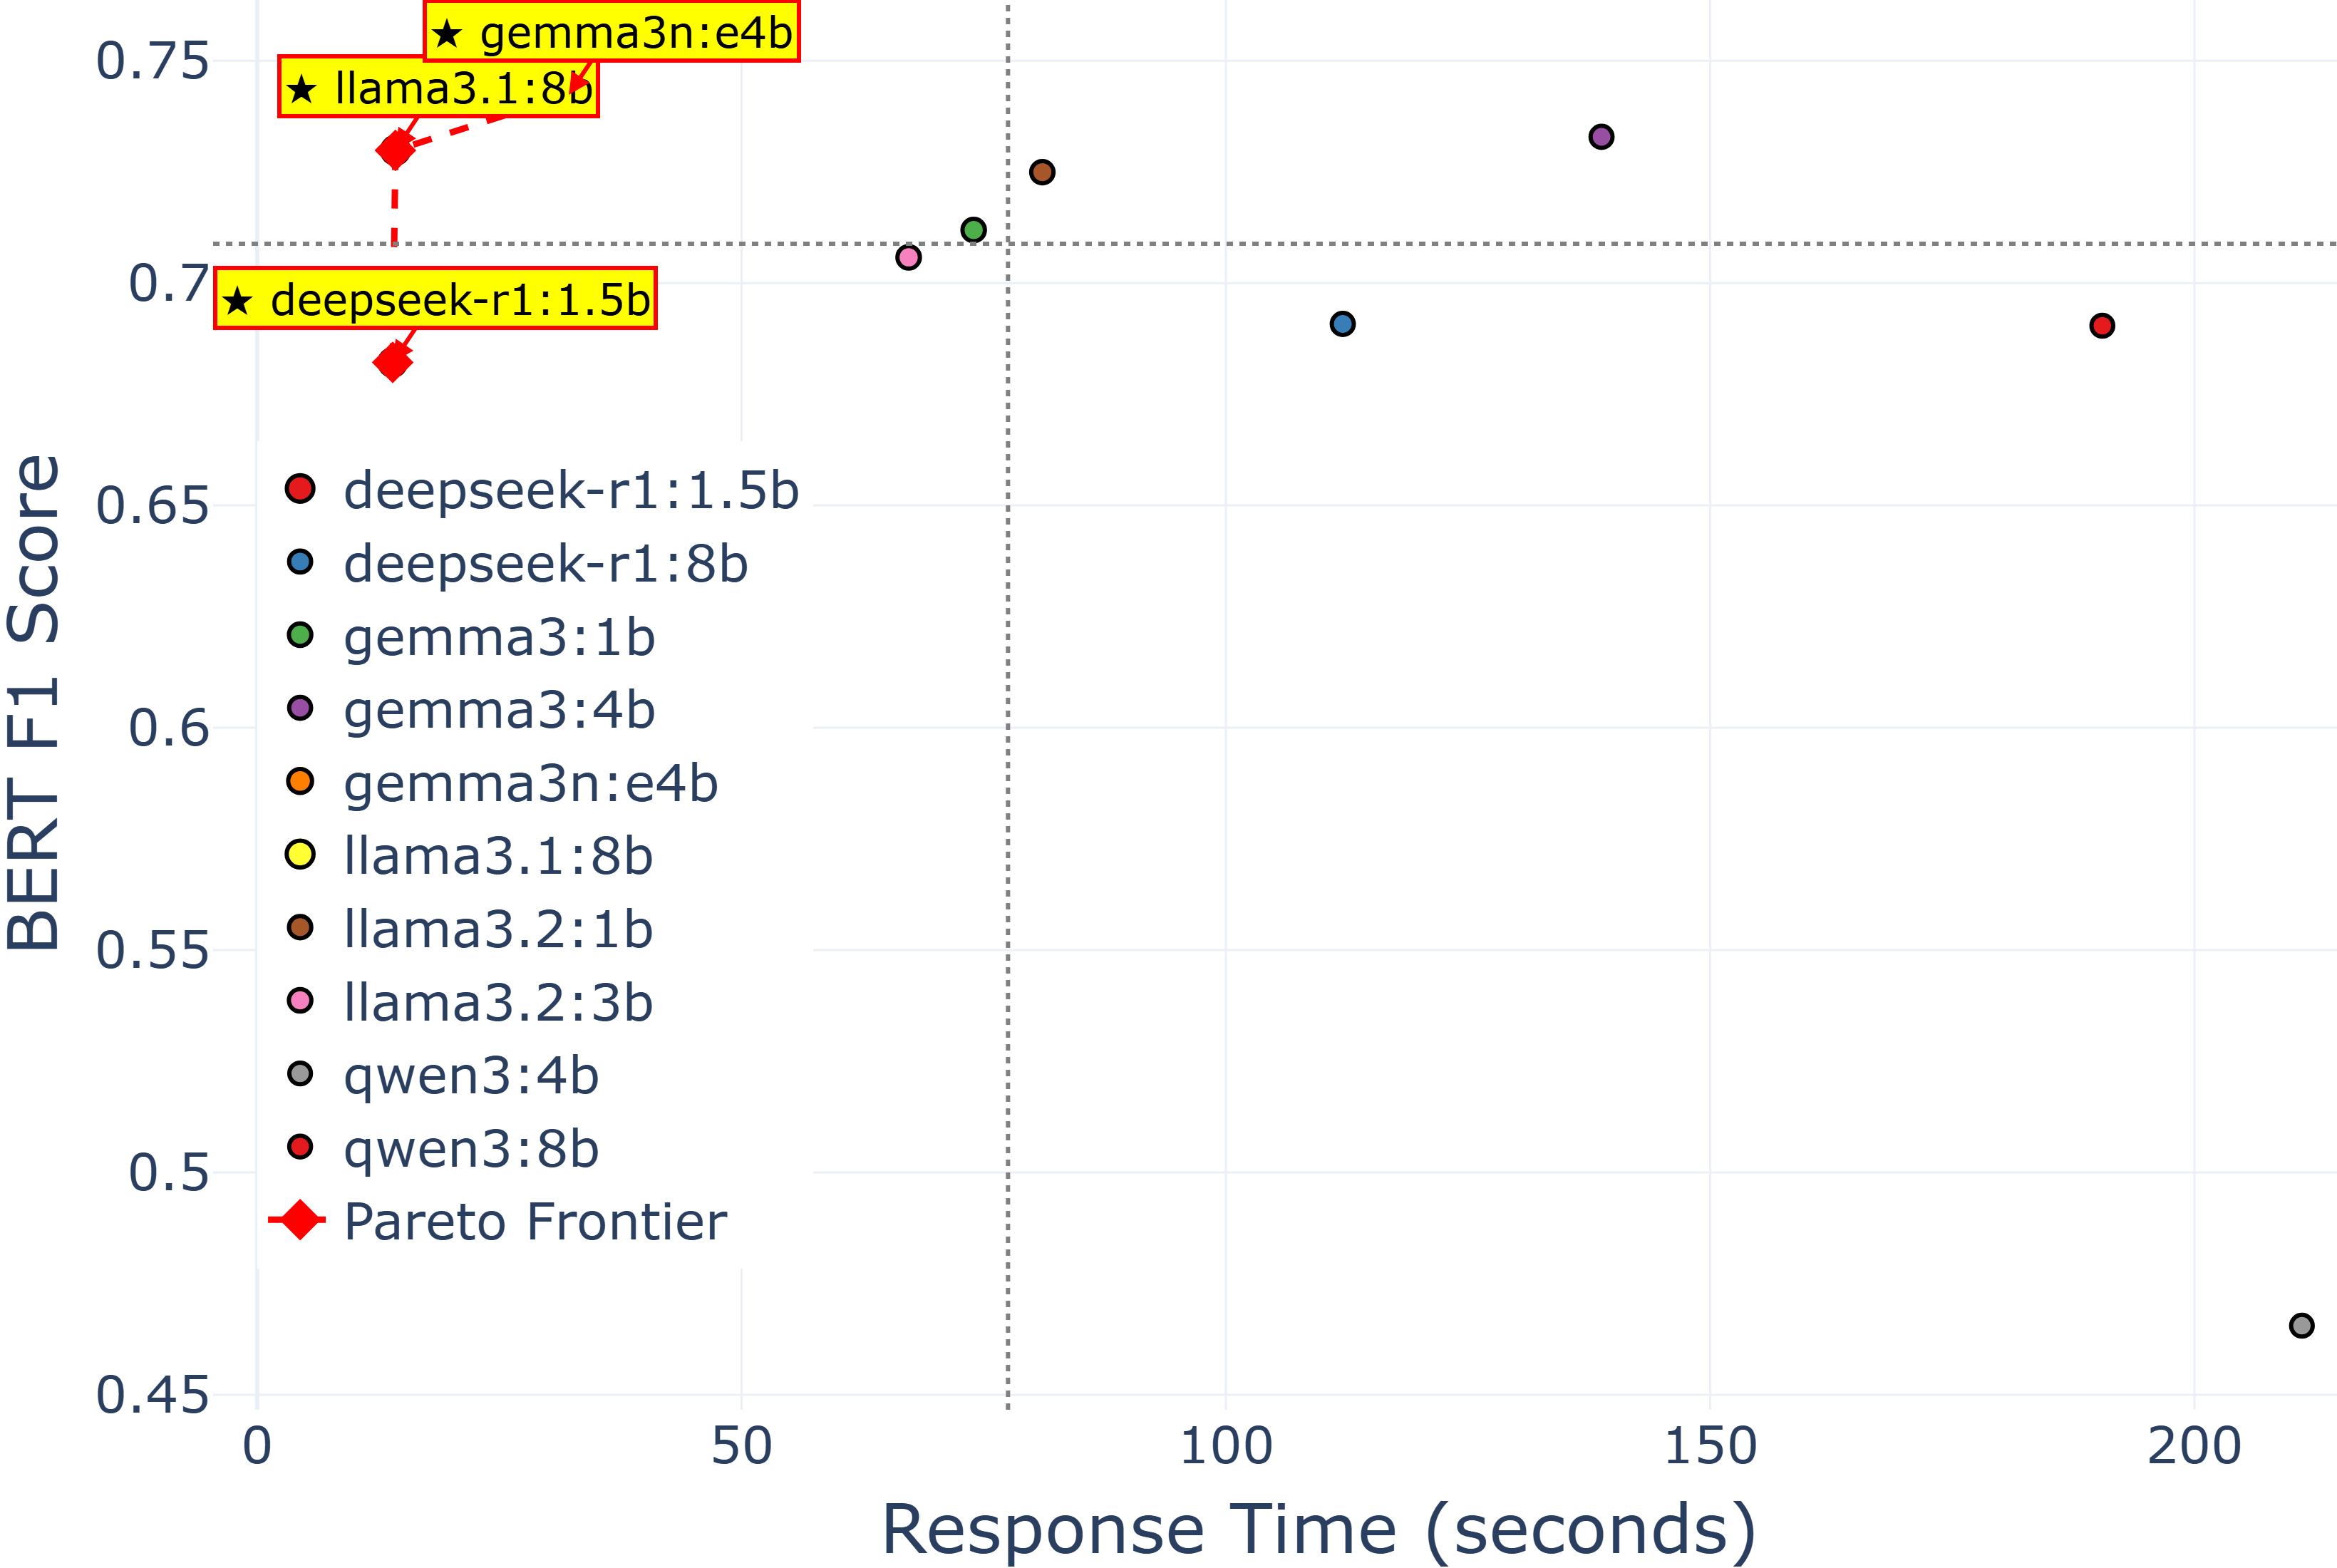
\includegraphics[width=\linewidth]{images/03_speed_quality_efficiency.png}
    \caption{Speed Quality Efficiency}
    \label{fig:eval_speed_quality}
  \end{minipage}
\end{figure}


Technical evaluation employed BERTScore precision, recall, and F1 to measure semantic similarity with reference answers.
As shown in Fig.~\ref{fig:eval_precision_recall}, the upper-right cluster contains the most reliable small- and medium-sized models, with precision between $0.60$–$0.75$ and recall between $0.70$–$0.76$. \texttt{gemma3n:e4b} achieved the highest precision ($0.75$) with recall $0.74$.
\texttt{Gemma3:4b} and \texttt{llama3.1:8b} exhibited similar performance, while \texttt{llama3.1:1b} and \texttt{llama3.2:3b} favored recall over precision.
\texttt{Deepseek-r1:1.5b}, \texttt{deepseek-r1:8b}, and \texttt{qwen3:8b} performed moderately (precision $0.62$–$0.64$, recall $\approx 0.75$).
\texttt{Qwen3:4b} was a clear outlier with substantially lower scores (precision $0.43$, recall $0.51$).

% \begin{figure}[!htbp]
%   \centering
%   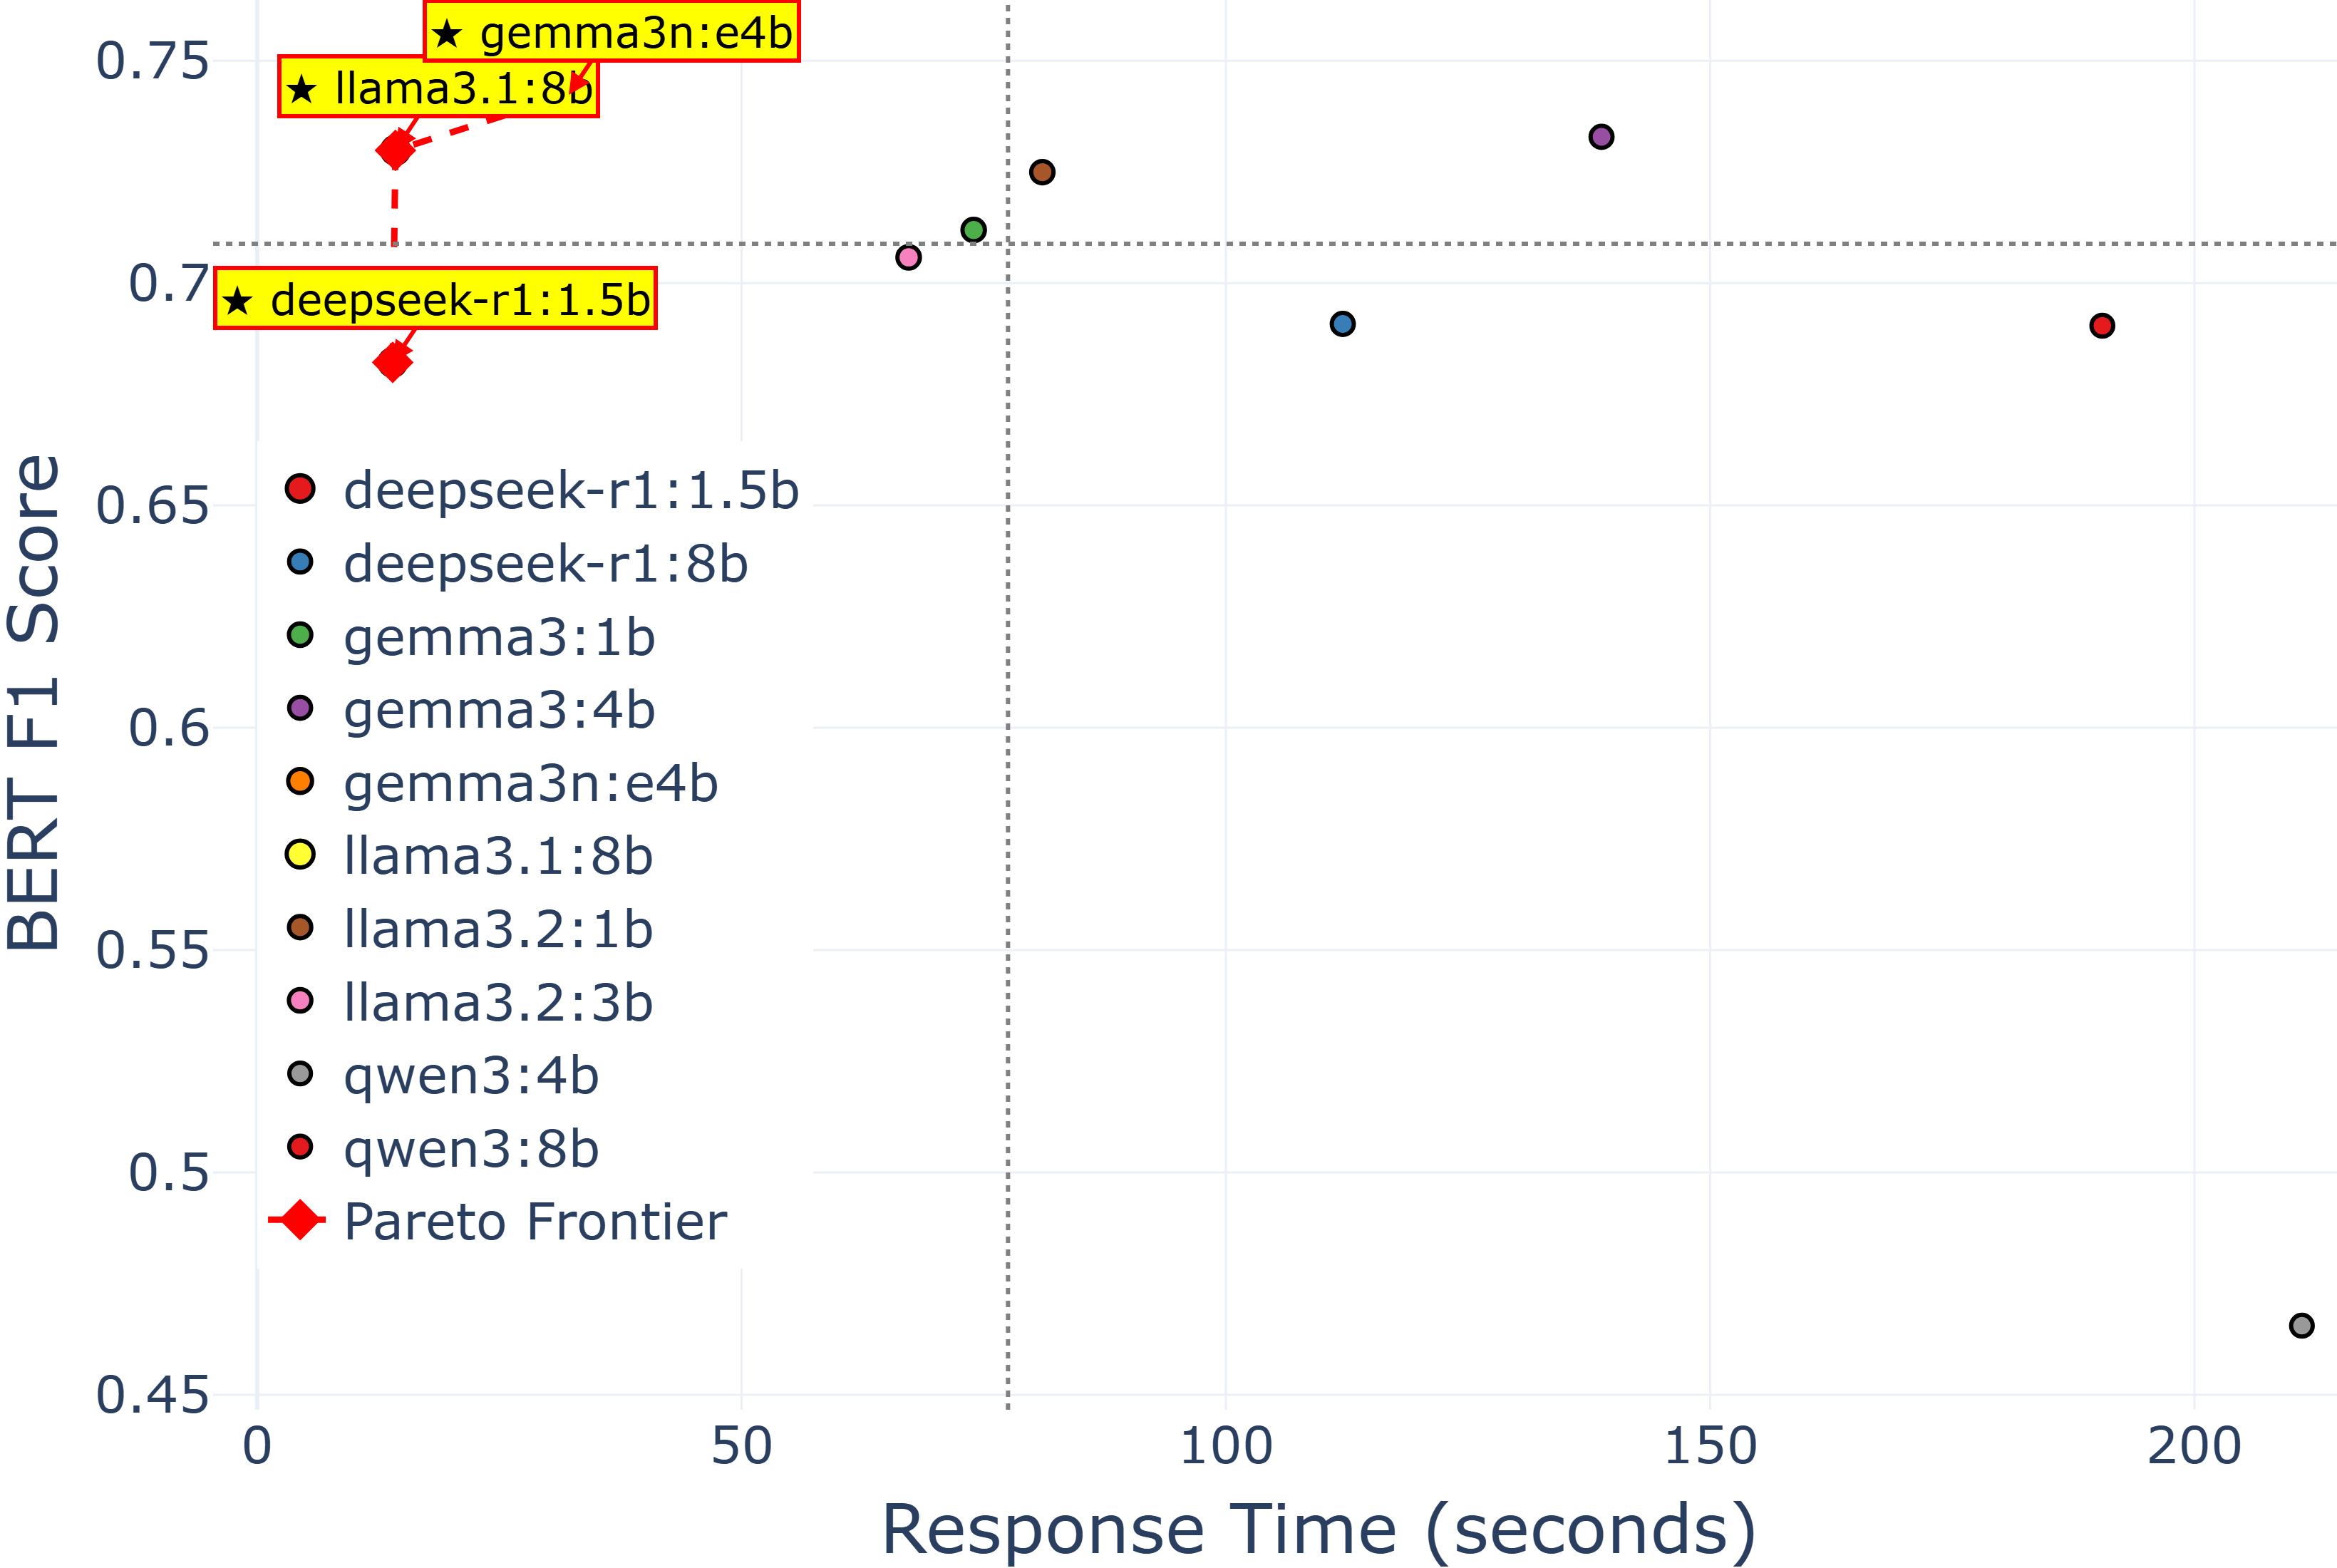
\includegraphics[width=\textwidth]{images/03_speed_quality_efficiency.png}
%   \caption{Speed Quality Efficiency}
%   \label{fig:eval_speed_quality}
% \end{figure}

Fig.~\ref{fig:eval_speed_quality} relates BERT F1 to query response time. Dashed guides indicate a latency threshold ($\sim 80$s) and a quality bar (F1 $\sim 0.71$). The target zone lies in the upper-left quadrant. \texttt{gemma3n:e4b} and \texttt{llama3.1:8b} were Pareto-optimal~\cite{b29}, achieving strong accuracy (F1 $0.74$–$0.75$) with moderate latency ($\sim 30$s). \texttt{deepseek-r1:1.5b} was the fastest ($15$–$20$s) but less accurate (F1 $0.69$–$0.70$). \texttt{gemma3:4b} reached F1 $\sim 0.73$ at much higher latency ($\sim 145$s). In contrast, \texttt{qwen3:8b} and \texttt{deepseek-r1:8b} fell below both thresholds, while \texttt{qwen3:4b} again underperformed. Overall, \texttt{gemma3n:e4b} and \texttt{llama3.1:8b} provided the best balance, with \texttt{deepseek-r1:1.5b} offering a low-latency alternative when moderate accuracy is acceptable.

\begin{figure}[!t]
  \centering
  \begin{subfigure}[t]{0.48\columnwidth}
    \centering
    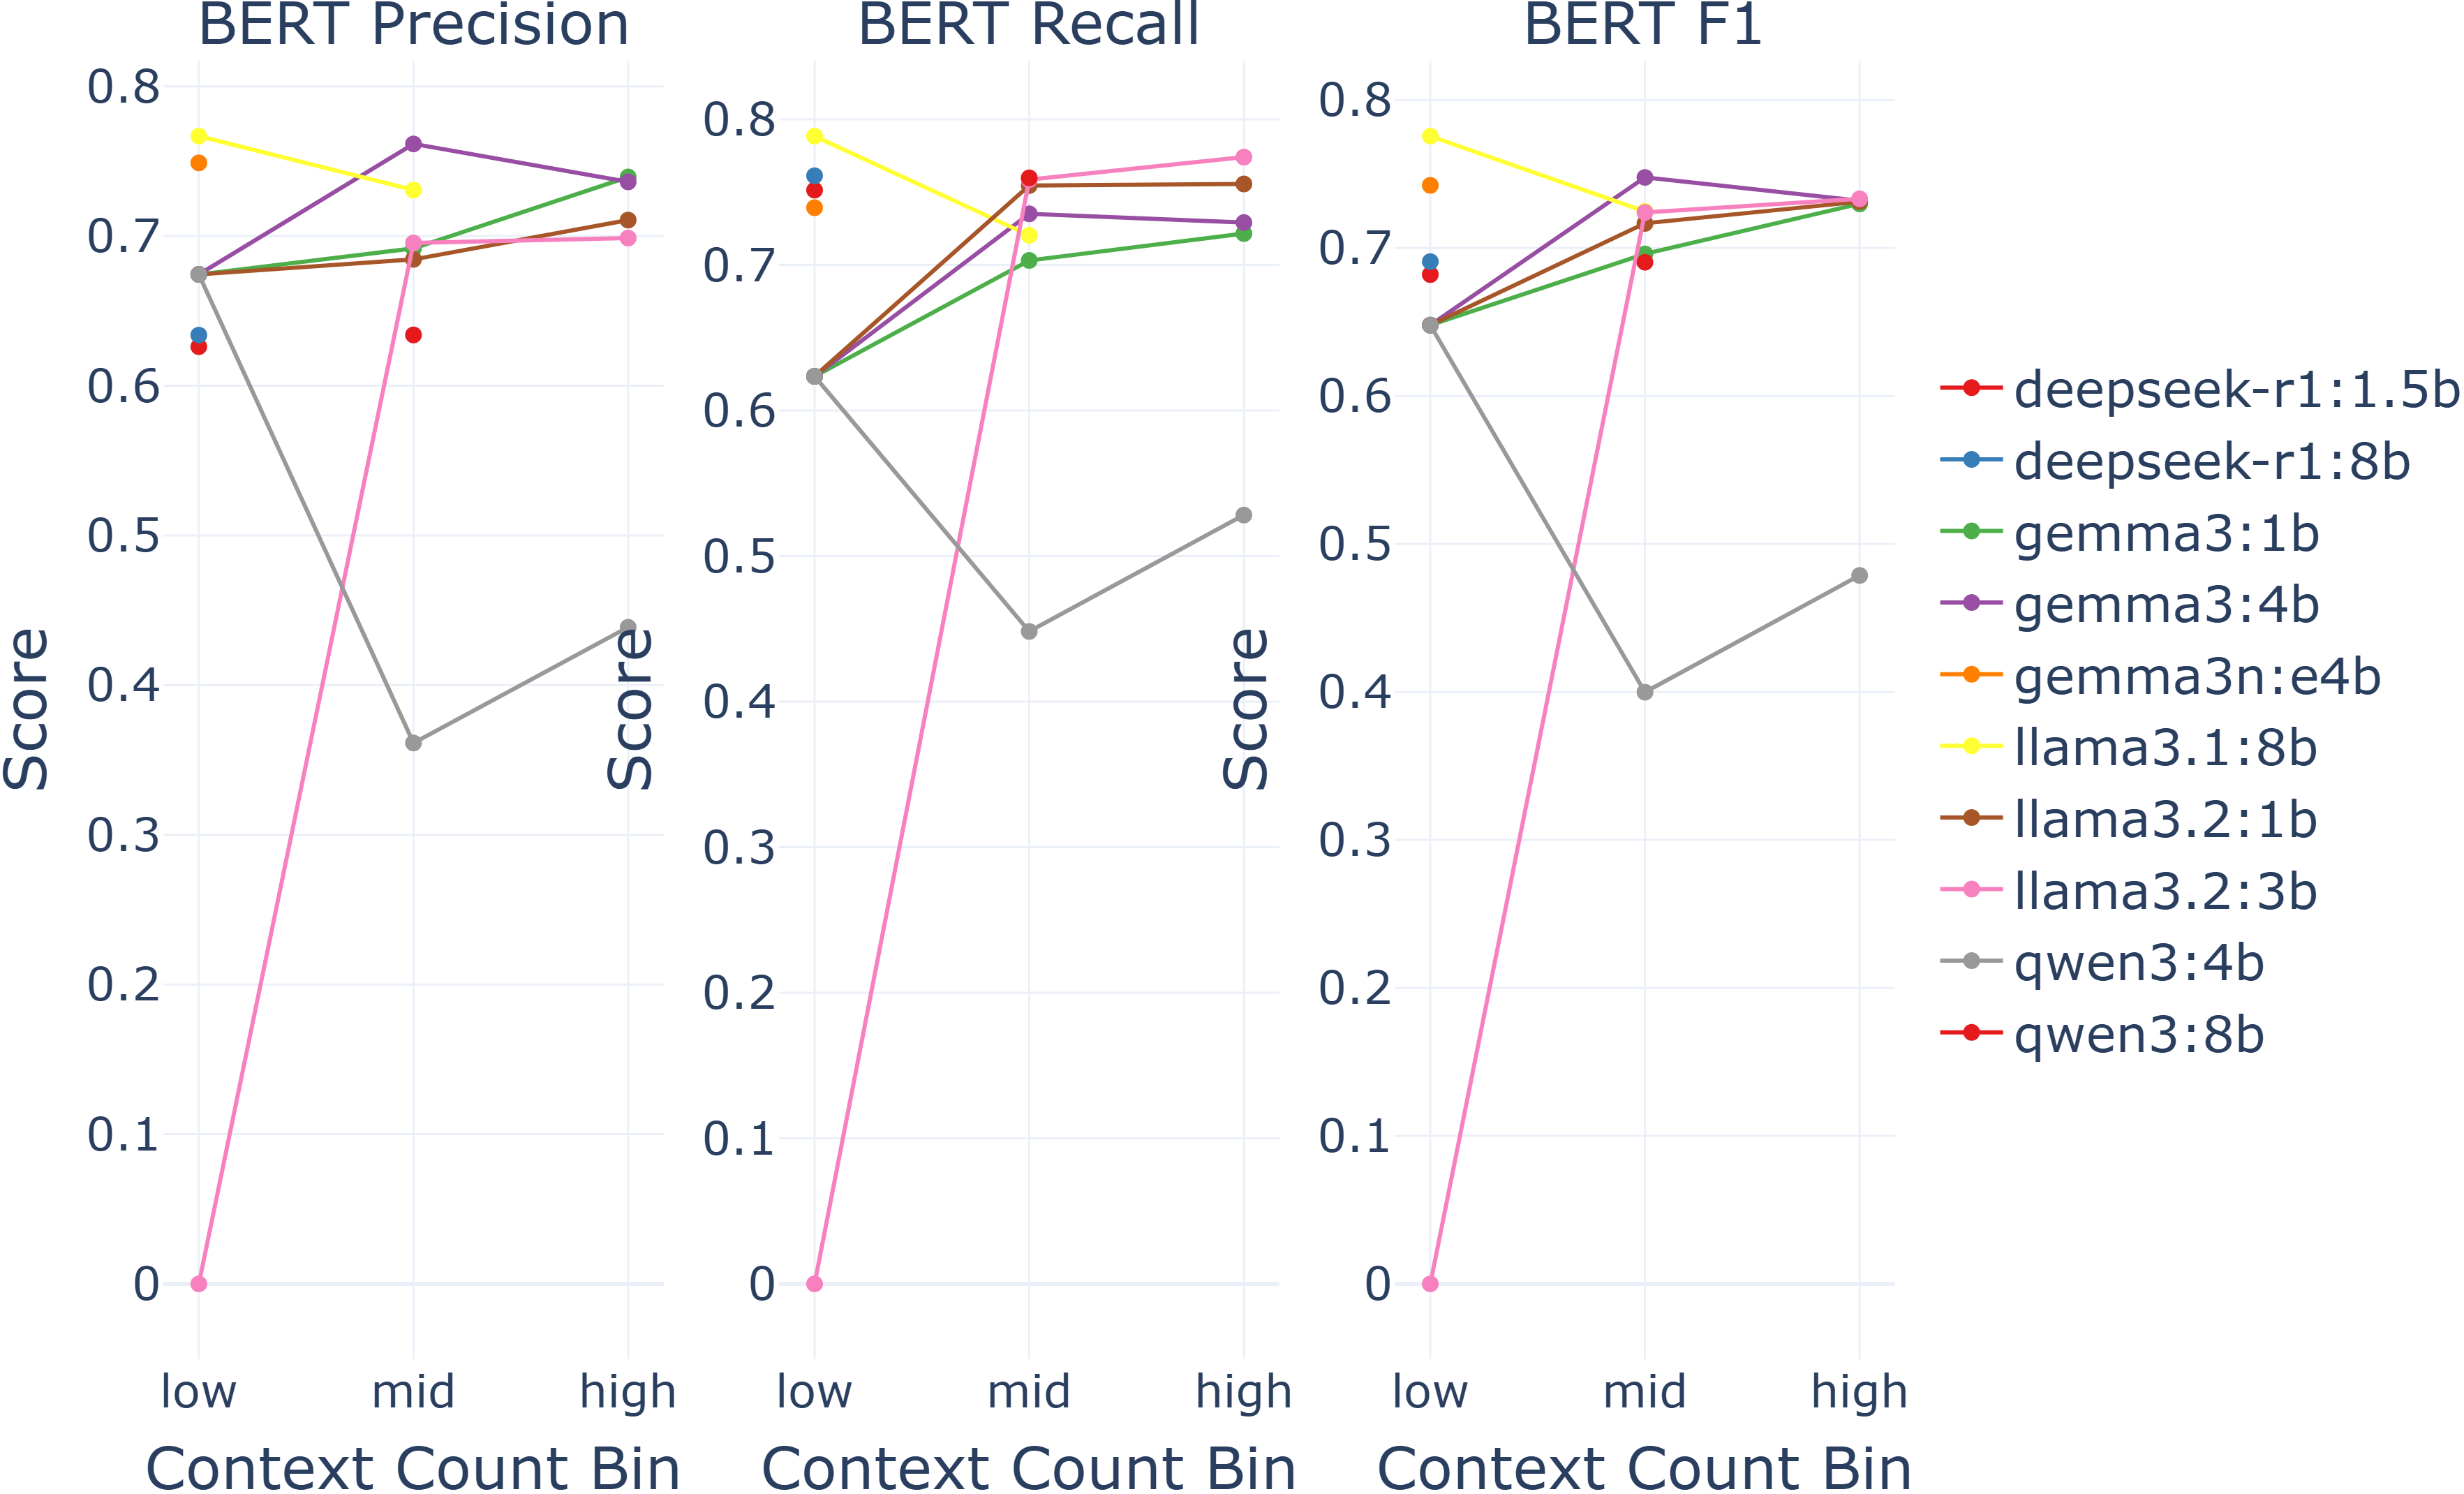
\includegraphics[width=\linewidth]{images/04_reading_progress_robustness.png}
    \caption{Reading Progress Robustness}
    \label{fig:eval_reading_progress_robustness}
  \end{subfigure}\hfill
  \begin{subfigure}[t]{0.48\columnwidth}
    \centering
    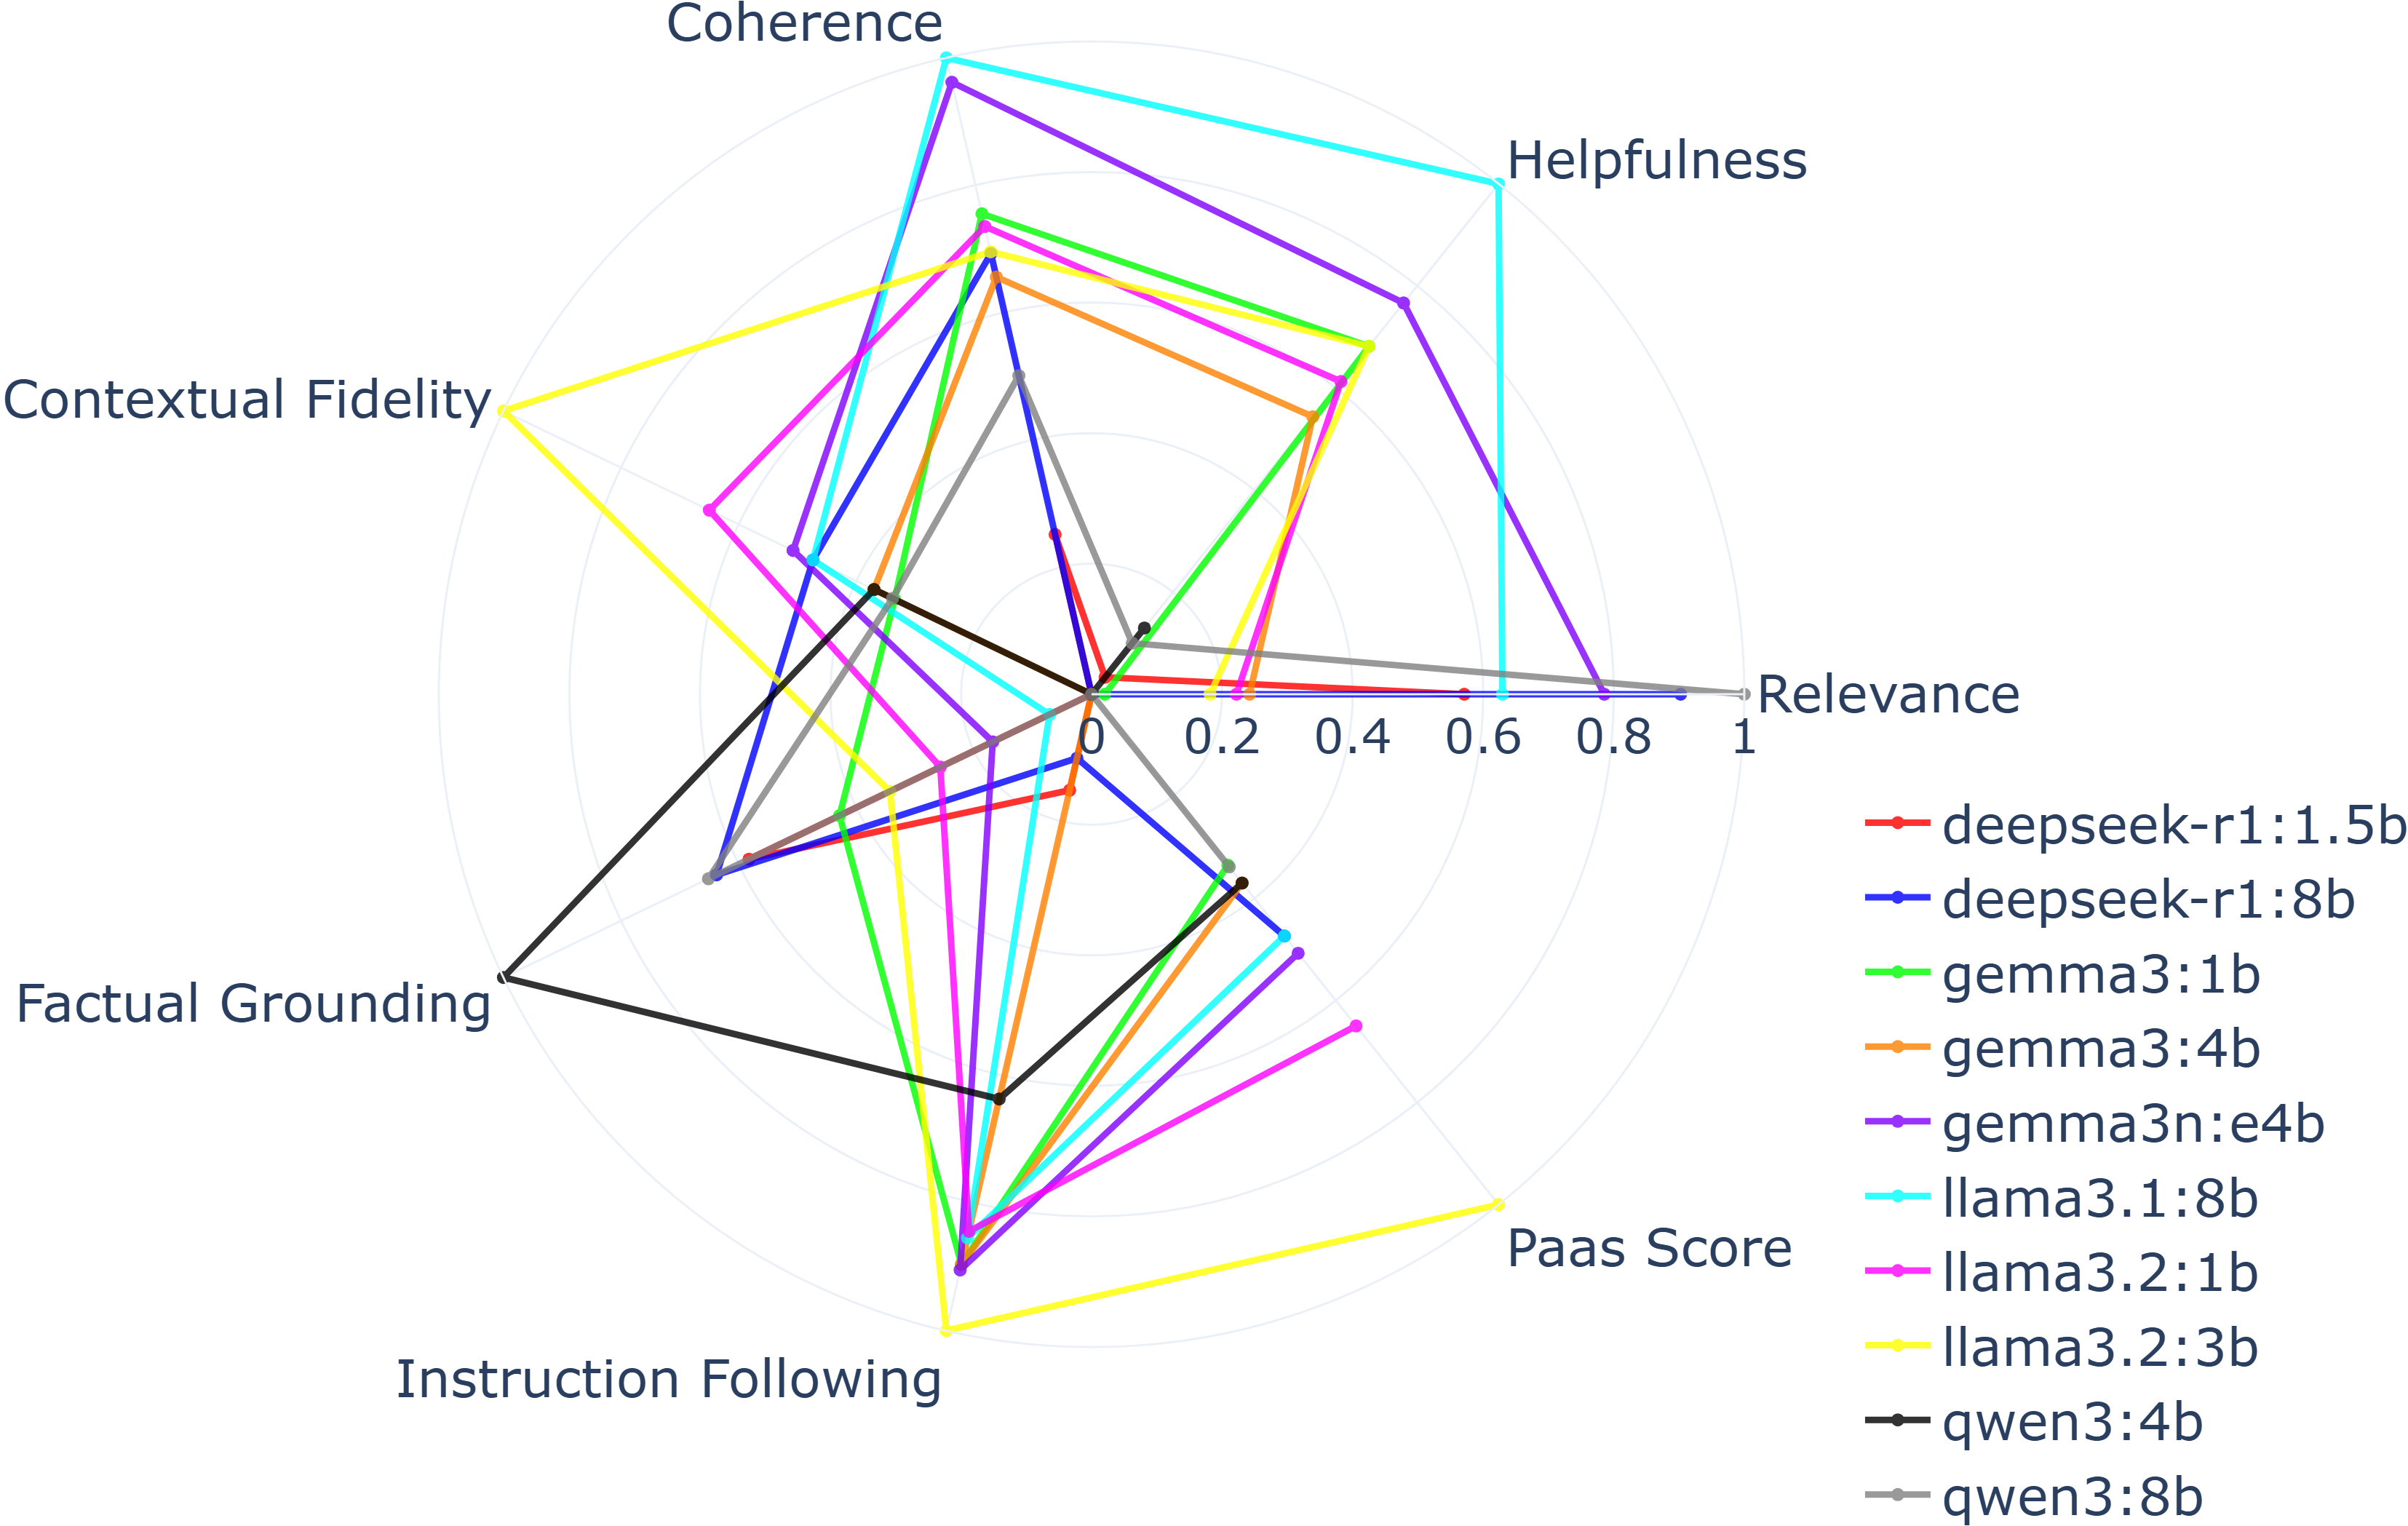
\includegraphics[width=\linewidth]{images/06_holistic_quality_radar.png}
    \caption{Qualitative Metric}
    \label{fig:eval_qualitative_metric}
  \end{subfigure}
  \caption{Robustness and Qualitative Radar}
  \label{fig:eval_bundle}
\end{figure}




Fig.~\ref{fig:eval_reading_progress_robustness} shows performance across progress bins: Low (1–2 passages), Mid (3–4), and High (5–6). Missing markers indicate that no items fell into a given bin due to either retrieval limitations or runner/API errors. \texttt{gemma3n:e4b}, \texttt{gemma3:4b}, and \texttt{llama3.1:8b} remained stable across bins, with precision $0.73$–$0.77$, recall $0.71$–$0.76$, and F1 $0.73$–$0.75$. These results suggest that even with minimal evidence, the models produced reliable answers, and additional passages did not degrade quality. \texttt{deepseek-r1:1.5b} and \texttt{deepseek-r1:8b} tracked slightly below but consistently across bins. By contrast, \texttt{qwen3:4b} showed a sharp decline at Mid (F1 $\sim 0.40$), recovering only partially at High (F1 $0.47$–$0.52$). \texttt{llama3.2:3b} produced no Low bin results).
But, when data was available, its F1 aligned with the $\sim 0.74$ band.
Even with limited evidence (1–2 passages), models maintained stable F1, reflecting adherence to the instruction not to speculate.

For qualitative evaluation, we employed an LLM-as-judge framework (Fig.~\ref{fig:eval_qualitative_metric}) across five dimensions: contextual fidelity, relevance, helpfulness, coherence, and instruction following. This approach provided a human-like assessment of response quality while ensuring evaluation consistency. The radar plots reveal that \texttt{gemma3n:e4b} and \texttt{llama3.1:8b} achieve consistently high scores across most dimensions, especially coherence and contextual fidelity, aligning with their strong precision–recall performance. \texttt{deepseek-r1:1.5b} delivers high instruction following but lags in coherence and helpfulness, reflecting its lower BERT F1 despite faster responses. In contrast, \texttt{qwen3:4b} underperforms across all axes, particularly in factual grounding and coherence, consistent with its outlier status in quantitative metrics.
These findings inform that models with balanced technical accuracy also tend to produce more user-satisfactory outputs in qualitative dimensions.

Fig.~\ref{fig:eval_qualitative_metric} summarizes the judgments averaged over the benchmark dimensions.
\texttt{Llama3.1:8b} and \texttt{gemma3n:e4b} form the best overall shapes with high helpfulness, coherence, and instruction following and competing contextual fidelity.
\texttt{Llama3.2:3b} has a high instruction following and contextual fidelity (strong adherence to prompts and book grounding), but is weaker on relevance (consistent with occasional over-literal responses).
\texttt{Deepseek-r1:8b} scores high on relevance and factual grounding, but trials on helpfulness.
\texttt{Qwen3:4b} shows high factual grounding but an overall smaller polygon all around, matching its error profile and low precisions seen in the earlier diagrams.
Overall, these readings align with those of the quantitative metrics.
Models that are coherent and helpful also sit near the precision-recall frontier, while models with generation errors have visibly collapsed polygons.

% Among all the models tested, error analysis reveals failures across three models only.
% In \texttt{llama3.2:3b}, nearly all errors were API related, explaining the absence of data points at low progress levels. Meanwhile, \texttt{qwen3:4b} exhibited primarily generation errors with a small tail of insufficient context, consistent with its lower precision and F1 scores elsewhere.
% These results, among many things, primarily show that there is a distinction between retrieval-related weaknesses and system-level execution errors.